Multi-valued model checking techniques, such as~\cite{bruns1999model,bruns2000model,gurfinkel2003multi,bruns2004MCmultivalued,DBLP:conf/fm/MenghiSG16}, have been proposed to support the verification of models that are \emph{partial}, i.e.,  their state space is not fully specified.
Three-valued model checking is a multi-valued model checking technique that extends classical two-valued model checking by possibly returning an additional \emph{maybe} value.
More precisely, it returns  \emph{true} if the property definitely holds, \emph{false} if it definitely does not hold,  \emph{maybe} otherwise.




In the classical context of two-valued model checking, although a sample violating behavior (a counterexample) is normally returned when the property is violated, no equally useful insight is provided if the property holds. 
In practice, it would be useful to receive a formal explanation of the reason \emph{why} the system satisfies the property.
To achieve this goal, the model checking framework can be equipped with a theorem prover that formally justifies why model checking has failed in the search of a counterexample.
Theorem proving algorithms have been developed for fully specified models~\cite{peled2001falsification,peled2001model}, but no known similar approach deals with partial models.

The ability to deal with partial models has a strong practical motivation. Software development often proceeds in an iterative and incremental fashion. Designers may start by providing an initial, high-level version of the model, which is iteratively narrowed down as design progresses and uncertainties are removed.
Whenever the result of verification  is \emph{true} or \emph{maybe}, the proof can guide the designer throughout the refinement process, and confirm the correctness of the design choices already performed. 
In some cases, the proof may even implicitly suggest that actually the property does not capture the intended correctness condition, and it should be modified.
For this reason, the integration of theorem proving techniques and multi-valued model checking can guide the designer towards the development of a correct model.

This paper proposes \NAME , a THRee valued Integrated Verification framEwork for partial models.
\NAME\ enriches model checking for partial models with theorem proving.
Theorem proving is used when a \emph{true} or a \emph{maybe} value is returned by the model checker to justify why the verified system \emph{definitely}  or \emph{possibly} satisfies the property of interest.
%Whenever the property \emph{definitely holds}, the deductive verification approach proves that neither a definitely violating nor a possibly violating behavior can be found in the current instance of the model.
%If the property \emph{possibly holds}, the model checker returns a possible counterexample, which describes a possible behavior that violates the property. 
%In addition, the deductive verification engine returns to the designer a proof that specifies why a violating behavior cannot be found in the current model.
%Finally, whenever the property \emph{does not hold}, a counterexample is returned, which specifies a violating behavior.
In addition to the general framework, we present  a specific instance of \NAME\ useful for applications, which considers models described as Partial Kripke Structures (PKSs)~\cite{bruns1999model} and properties expressed as Linear Temporal Logic (LTL)~\cite{pnueli1977temporal} formulae.
The instance is based on the three-valued LTL semantics~\cite{bruns1999model}.
To successfully integrate model checking and theorem proving we customize the theorem proving framework (based on deductive verification) proposed in~\cite{peled2001model} to support PKSs and LTL formulae.

We consider the applicability of \NAME\  w.r.t.  \emph{three-valued}~\cite{bruns1999model} and  \emph{thorough}~\cite{bruns2000model} LTL semantics. 
We also discuss its applicability in the case of \emph{self-minimizing}~\cite{godefroid2005MCvsGMC} LTL formulae, which are known to represent a practically relevant subset of LTL formulae~\cite{antonik2006efficient}. 
We evaluate the benefits of the framework on an example by simulating  the design of a medical software critical component~\cite{arcaini2015formal}.
A discussion on the use of \NAME\ in real world scenarios concludes the evaluation.




\begin{figure}[t]
 \centering
\begin{tikzpicture}[scale=0.33] %[x={10.0pt},y={10.0pt}]

\node [state, initial, initial text={},initial where=above](s_0)
[label={
[align=center,yshift=0.1cm]
%above:
% 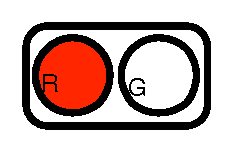
\includegraphics[width=50pt]{images/Red.pdf}
%$\boldsymbol{\overline{green}=T}$\\
$g=\color{black}\bot$\\
$r=\LTLtrue$
}] 
{$s_0$};   


\node[state] (s_1) 
[left=of s_0,
label={
[align=center,yshift=0.1cm]
%above:
% \includegraphics[width=50pt]{images/Green.pdf}
%$\boldsymbol{\overline{green}=F}$\\
$g=\color{black}\LTLtrue$\\
$r=\bot$
}]  
{$s_1$};

\node[state] (s_2) 
[right=of s_0,
label={
[align=center,yshift=0.1cm]
%above:
% \includegraphics[width=50pt]{images/Bo.pdf}
%$\boldsymbol{\overline{green}=\bot}$\\
$g=\color{black}?$\\
$r=?$
}]  
{$s_2$};


\path[->]      
(s_0) edge [bend left] node [above]{} (s_1) 
(s_1) edge [bend left] node [above]{} (s_0)
(s_0) edge [bend left] node [above]{} (s_2)
(s_2) edge [bend left] node [above]{} (s_0);   

\end{tikzpicture}
\caption{System model $M$}
\label{fig:modelmot}
\end{figure}


\textbf{Running example}. \emph{We consider a  simple grade crossing semaphore.
We assume that the designer has identified three simple properties:
\begin{enumerate*}[label={(\arabic*)}]
\item $Red$ lights up infinitely often -- formalized as $\phi_1=\LTLglobally\LTLfinally red$.
\item $Green$ lights up infinitely often -- formalized as $\phi_2=\LTLglobally\LTLfinally green$.
\item When the light is $red$, it will always be $green$ -- formalized as $\phi_3=\LTLglobally (red \LTLimplication \LTLglobally green)$.
\end{enumerate*}
Note that $\phi_3$ is deliberately wrong %(i.e., it does not capture the desired behavior).
and will be used later to discuss the application of \NAME .\hfill
\break
Starting from this specification, a designer might initially propose the partially specified model of the semaphore shown in Figure~\ref{fig:modelmot}. Each state is associated with the values of the propositions $g$ and $r$ (denoting $green$ and $red$) holding in that state, which specify whether the green and the red lights are on or off.
For example, in state $s_0$ the red light is on ($r=\LTLtrue$) while the green is off ($g=\LTLfalse$).
Instead,  $s_2$ is a state to which the semaphore may be brought, for instance by a manual command. 
The designer still has to choose whether, in this state, the green and red lights should be on or off.
This is indicated by associating the value $?$ to the propositions $g$ and $r$.
The designer might refine the model by setting $g$ and $r$ to either $\LTLtrue$ or $\LTLfalse$ in $s_2$.}

\textbf{Related work.}
Three-valued~\cite{larsen1988modal,godefroid2001abstraction,bruns1999model,bruns2000model,godefroid2011ltl} and multi-valued~\cite{gurfinkel2003multi,bruns2004MCmultivalued} model checking supports verification of partial models. 
Different model checking techniques have been developed depending on the modeling formalisms.
For example, several papers  focus on Partial Kripke Structures (e.g.,~\cite{bruns1999model,bruns2000model,godefroid2011ltl,gurfinkel2003multi,bruns2004MCmultivalued}), others on Modal Transition Systems (e.g.,~\cite{larsen1988modal,godefroid2001abstraction}). 
However, to the best of our knowledge, none of these techniques has been combined with theorem proving.  

Theorem proving applies a set of techniques to try to establish the validity of a given formula (see~\cite{manna2012temporal}).
Some of these techniques (e.g., ~\cite{peled2001falsification,peled2001model,namjoshi2001certifying,cleaveland2002evidence,rajan1995integration}) exploit the state space generated by the model checker to explain why a property holds.
However, to the best of our knowledge, none of these approaches has been applied in a multi-valued context.


\textbf{Organization.}
Section~\ref{sec:preliminaries} contains background notations and algorithms.
%presents the background. notations and algorithms.
Section~\ref{sec:contribution} describes \NAME.
Section~\ref{sec:theoremProverAdapting} presents an instance of \NAME , that considers PKSs and LTL formulae. 
Section~\ref{sec:preliminaryEvaluation} evaluates the approach on an example.
Section~\ref{sec:discussion} discusses the applicability of \NAME\ in real world cases.
%Finally, Section~\ref{sec:conclusions} concludes the paper.
Section~\ref{sec:conclusions} concludes the paper.